\section{The DAQ System }
\label{sec:DAQ}

%%%%%%%%%%%%%%%%%%%%%%%%%%%%%%%%%%%%%%%%%%%%%%%%%%%%%%%%%%%%%%%%%%%%%%%%%%%%%%%%%%%%
%by MMdevi. Last modified July 2, 2017.
%%%%%%%%%%%%%%%%%%%%%%%%%%%%%%%%%%%%%%%%%%%%%%%%%%%%%%%%%%%%%%%%%%%%%%%%%%%%%%%%%%%%

The DAQ system consists of a heterogeneous system with both 
NIM and VME electronics modules, with the data readout being carried out 
through an optical link via a VME controller\footnote{CAEN V2718} and a 
PCIe card \footnote{CAEN A3818}. 

The schematic layout of the DAQ system is shown in Fig.~{\ref{Fig:DAQscheme}}. 
The PMTs are ramped up to +800V (the maximum is +900V) using a 24 channel VME high 
The raw electrical pulse output of the PMTs are denoted as S{\it i}(raw), where {\it i} = 1 -- 20. 
These raw pulses are then amplified and shaped using two photomultiplier preamplifiers 
\footnote{Phillips 776. 16 independent and direct-coupled amplifiers channels}. 
The preamplifier channels operates from DC to 275 MHz and produce two identical 
50 $\Omega$ non inverting FIFO outputs with voltage gains of 10. 
The amplified pulses are denoted as S{\it i} 
({\it i} = 1 -- 20). One of the two FIFO outputs from each channel is converted to a 
digital signal with an Analog to Digitizer converter \footnote{CAEN ADC V1742: Switched capacitor Digitizer}. 

%%%%%%%%%%%%%%%%%%%%%%%%%%%%%%%%%%%%%%%%%%%%%%%%%%%%%%%%%%%%%%%%%%%%%%%%%%
\begin{figure}[h]
   \centering
   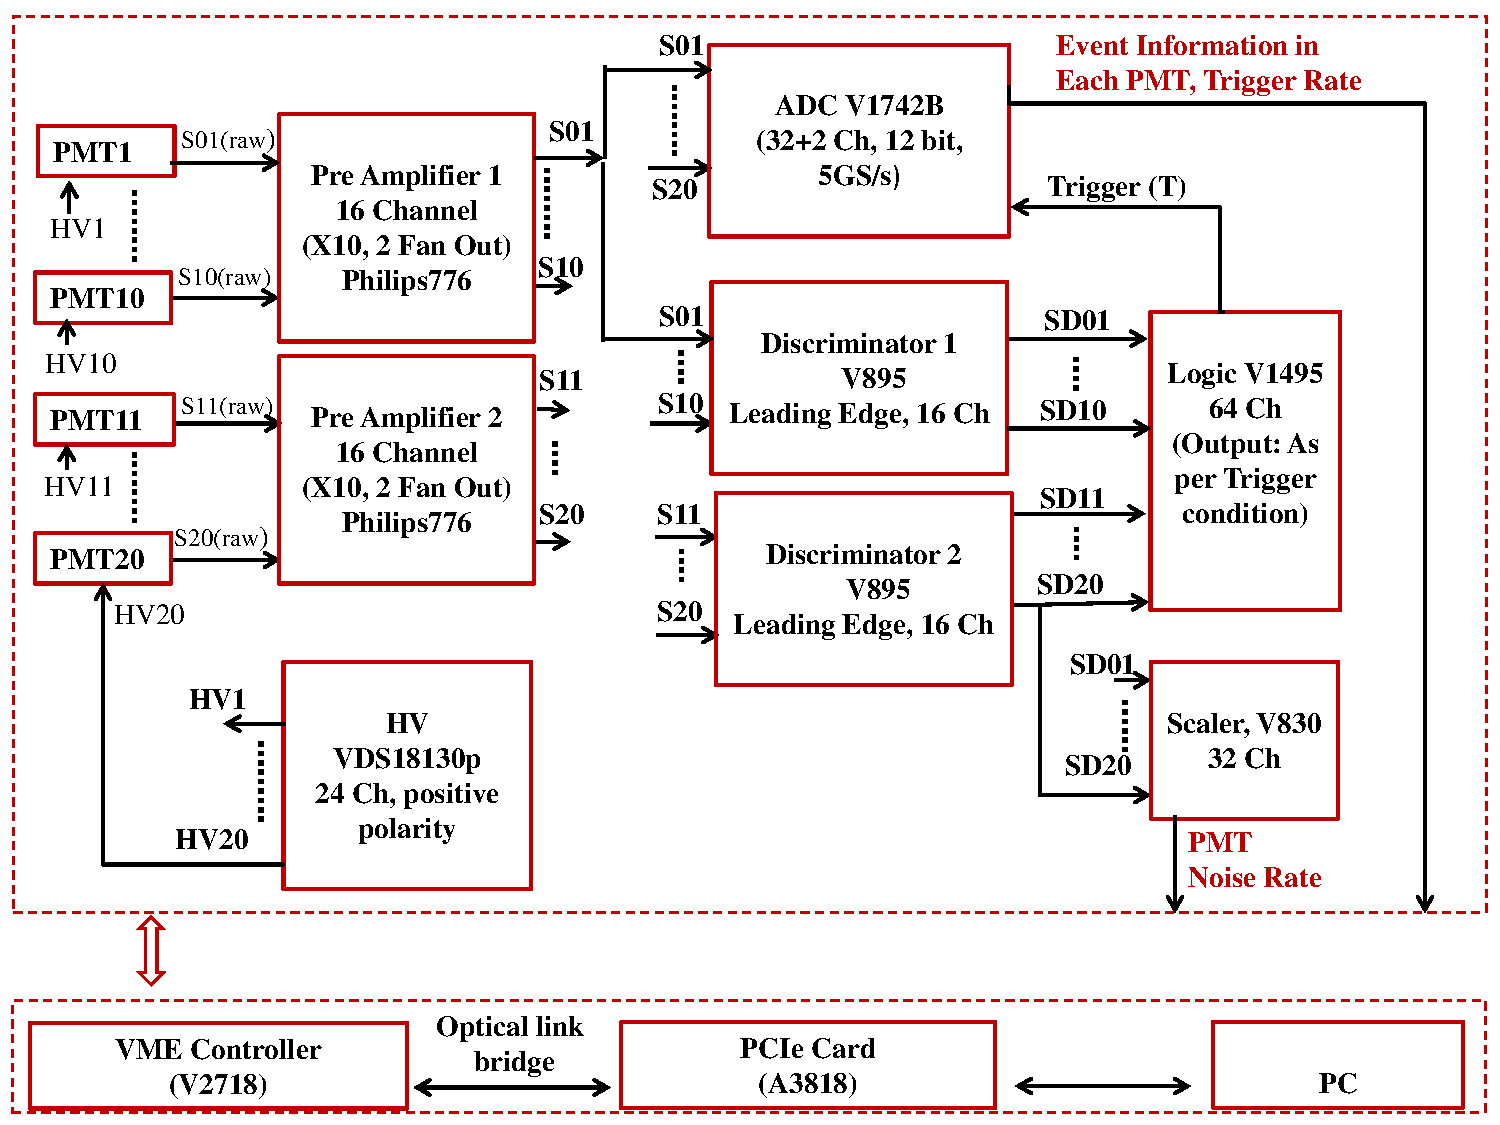
\includegraphics[width=0.85\textwidth]{DAQscheme.pdf}
   \caption{The schematic of the Data Acquisition System of DIREXENO. It 
        consists of 20 PMTs and the subsequent electronic channels to record 
        the events for an internal trigger generated by the coincidence of any 
        two PMTs in the system and also the PMT noise rate.}
   \label{Fig:DAQscheme}
\end{figure}
%%%%%%%%%%%%%%%%%%%%%%%%%%%%%%%%%%%%%%%%%%%%%%%%%%%%%%%%%%%%%%%%%%%%%%%%%%%

The schematic layout 
of the DAQ system is shown in Fig.~{\ref{Fig:DAQscheme}}. All the 20 PMTs 
are oriented in the holder assembly which was discussed in section \ref{subsubsec:sphere}. 
The PMTs are ramped up to +800V (the maximum is +900V) using a 24 channel 
VME high voltage distributor module \footnote{iseg VDS18130p : 24 independent channels with positive polarity}.  
The raw electrical pulse output of the PMTs are defined as S{\it i} (raw), where {\it i} = 1 -- 20. 
These raw pulses are then 
amplified and shaped using two photomultiplier preamplifiers \footnote{Phillips 776: 16 independent  and direct-coupled 
amplifiers channels}. The preamplifier channels operates from DC to 275 MHz and 
produce two identical 50 $\Omega$ non inverting outputs with voltage gains of 10. 
The amplified pulses as defined as S{\it i}, ({\it i} = 1 -- 20). One out of the 
two identical analog outputs from each channel is converted to a digital 
signal with an Analog to Digitizer converter \footnote{CAEN ADC V1742: 
32 channel switched capacitor Digitizer}. 


The ADC consists of two 12bit 5GS/s Switched capacitor Digitizer sections, 
each of them with 16+1 channels, based on DRS4 chip. The dynamic range of the input signal is 1 
Vpp with adjustable DC offset. This module can sample either bipolar or unipolar analog input 
signal within the dynamic range in a circular 
analog memory buffer, with default sampling frequency choices 5GS/s, 2.5 GS/s 
or 2 GS/s. As soon as a trigger signal reaches, all the analog memory 
buffers gets frozen and then gets digitized into a digital memory buffer 
with a 12 bit resolution. 

An intrinsic trigger is generated for the system, 
with the coincidence of any two out of the twenty PMTs. The second output from the 
preamplifier channels are converted to binary signals using two 16 channel leading 
Edge discriminator \footnote{CAEN V895}. In Fig.~\ref{Fig:DAQscheme}, the binary 
outputs from the discriminator are denoted as SD{\it i}, i= 1 -- 20. The SD{\it i} signals are then passed over to 
the logic module \footnote{CAEN V1495: FPGA based General purpose VME board} to obtain the trigger. The output of the logic operation is 
used to trigger the ADC. In order to record the PMT noise rate, the 
SD{\it i} signals are duplicated and fed to a scaler \footnote{CAEN V830: 16 channel}.

The PMT event information and the trigger rate are read from the ADC, while the Scaler 
records the PMT noise rate. The further analyses of the 
relevant events in the PMTs are carried out offline using an analysis 
framework.










%\clearpage %temporary TBC
